% questions.tex —— 2016 年·四川卷·理科 · 题目内容片段（无答案）
% 由 tools/generate_projects.py 依来源总账自 2016/2016_数学真题_四川理_试题.md 生成，勿手改（改源 MD 后重跑）


\gkpart{数学}

\begin{gktip}
\textbf{来源说明}：本题面依据固定源 PDF 两页 A3 页面逐题核对，原卷印刷页码 1019–1020。固定源不附答案；本文件仅为题面规范源。
\end{gktip}

\gkpart{一、选择题}

\begin{question}
\gkti{1}设集合 \(A=\{x\mid -2\leqslant x\leqslant 2\}\)，\(\mathbf{Z}\) 为整数集，则 \(A\cap\mathbf{Z}\) 中元素的个数是（　）

\begin{gkopts}(4)
\task （A）\(3\)
\task （B）\(4\)
\task （C）\(5\)
\task （D）\(6\)
\end{gkopts}

\end{question}
\begin{question}
\gkti{2}设 \(\mathrm{i}\) 为虚数单位，则 \((x+\mathrm{i})^{6}\) 的展开式中含 \(x^{4}\) 的项为（　）

\begin{gkopts}(2)
\task （A）\(-15x^{4}\)
\task （B）\(15x^{4}\)
\task （C）\(-20\mathrm{i}x^{4}\)
\task （D）\(20\mathrm{i}x^{4}\)
\end{gkopts}

\end{question}
\begin{question}
\gkti{3}为了得到函数 \(y=\sin\left(2x-\dfrac{\pi}{3}\right)\) 的图象，只需把函数 \(y=\sin 2x\) 的图象上所有的点（　）

（A）向左平行移动 \(\dfrac{\pi}{3}\) 个单位长度　（B）向右平行移动 \(\dfrac{\pi}{3}\) 个单位长度

（C）向左平行移动 \(\dfrac{\pi}{6}\) 个单位长度　（D）向右平行移动 \(\dfrac{\pi}{6}\) 个单位长度

\end{question}
\begin{question}
\gkti{4}用数字 \(1,2,3,4,5\) 组成没有重复数字的五位数，其中奇数的个数为（　）

\begin{gkopts}(2)
\task （A）\(24\)
\task （B）\(48\)
\task （C）\(60\)
\task （D）\(72\)
\end{gkopts}

\end{question}
\begin{question}
\gkti{5}公司为激励创新，计划逐年加大研发资金投入。若该公司 \(2015\) 年全年投入研发资金 \(130\) 万元，在此基础上，每年投入的研发资金比上一年增长 12\%，则该公司全年投入的研发资金开始超过 \(200\) 万元的年份是（　）

（参考数据：\(\lg 1.12\approx 0.05\)，\(\lg 1.3\approx 0.11\)，\(\lg 2\approx 0.30\)）

\begin{gkopts}(2)
\task （A）\(2018\) 年
\task （B）\(2019\) 年
\task （C）\(2020\) 年
\task （D）\(2021\) 年
\end{gkopts}

\Needspace{0.4\textheight}
\end{question}
\begin{question}
\gkti{6}秦九韶是我国南宋时期的数学家，普州（现四川省安岳县）人，他在所著的《数书九章》中提出的多项式求值的秦九韶算法，至今仍是比较先进的算法。如图所示的程序框图给出了利用秦九韶算法求某多项式值的一个实例，若输入 \(n,x\) 的值分别为 \(3,2\)，则输出 \(v\) 的值为（　）
\nopagebreak[4]
\begin{center}% 第 6 题程序框图（秦九韶算法）：按固定源 PDF 逐框重绘（9 框；回边在主干右侧）。
% 循环体次序（易错点，矢量路径逐段核对）：「是」分支自菱形右顶点折出，先入 \(v=vx+i\)，
% 再上行入 \(i=i-1\)，最后由该框左边缘水平折回主干（箭头指向主干，T 形汇入）。
% 主干 x=0；回边列 x=2.44；join 在 \(i=n-1\) 与菱形之间的主干上。
\begin{tikzpicture}[>=stealth,every node/.style={font=\small},
  term/.style={draw,rounded corners,minimum width=1.5cm,minimum height=5.5mm},
  box/.style={draw,minimum height=5.5mm,inner xsep=4pt},
  io/.style={draw,trapezium,trapezium left angle=70,trapezium right angle=110,minimum width=1.8cm,minimum height=5.5mm},
  decision/.style={draw,diamond,aspect=4,minimum width=2.7cm,inner sep=0pt}]
\node[term] (start) at (0,0) {开始};
\node[io] (input) at (0,-1.10) {输入 \(n,x\)};
\node[box] (v1) at (0,-2.15) {\(v=1\)};
\node[box] (in1) at (0,-3.16) {\(i=n-1\)};
\node[decision] (test) at (0,-5.86) {\(i\geqslant 0?\)};
\node[io] (out) at (0,-7.01) {输出 \(v\)};
\node[term] (end) at (0,-8.11) {结束};
\node[box] (iim1) at (2.44,-3.89) {\(i=i-1\)};
\node[box] (vvx) at (2.44,-4.92) {\(v=vx+i\)};
\coordinate (join) at (0,-3.89);
\draw[->] (start)--(input);
\draw[->] (input)--(v1);
\draw[->] (v1)--(in1);
\draw[->] (in1)--(test);
\draw[->] (test.south)--node[right,xshift=2pt]{否}(out.north);
\draw[->] (out)--(end);
\draw[->] (test.east) -| node[below,pos=0.3]{是} (vvx.south);
\draw[->] (vvx.north)--(iim1.south);
\draw[->] (iim1.west)--(join);
\end{tikzpicture}
\end{center}
\nopagebreak[4]
\begin{gkopts}(2)
\task （A）\(9\)
\task （B）\(18\)
\task （C）\(20\)
\task （D）\(35\)
\end{gkopts}

\end{question}
\begin{question}
\gkti{7}设 \(p\)：实数 \(x,y\) 满足 \((x-1)^{2}+(y-1)^{2}\leqslant 2\)，\(q\)：实数 \(x,y\) 满足

\nopagebreak[4]
\[
\begin{cases}
y\geqslant x-1,\\
y\geqslant 1-x,\\
y\leqslant 1.
\end{cases}
\]

则 \(p\) 是 \(q\) 的（　）

（A）必要不充分条件　（B）充分不必要条件

（C）充要条件　（D）既不充分也不必要条件

\end{question}
\begin{question}
\gkti{8}设 \(O\) 为坐标原点，\(P\) 是以 \(F\) 为焦点的抛物线 \(y^{2}=2px\)（\(p>0\)）上任意一点，\(M\) 是线段 \(PF\) 上的点，且 \(|PM|=2|MF|\)，则直线 \(OM\) 的斜率的最大值为（　）

\begin{gkopts}(2)
\task （A）\(\dfrac{\sqrt{3}}{3}\)
\task （B）\(\dfrac{2}{3}\)
\task （C）\(\dfrac{\sqrt{2}}{2}\)
\task （D）\(1\)
\end{gkopts}

\end{question}
\begin{question}
\gkti{9}设直线 \(l_{1},l_{2}\) 分别是函数

\nopagebreak[4]
\[
f(x)=\begin{cases}
-\ln x, & 0<x<1,\\
\ln x, & x>1,
\end{cases}
\]

图象上点 \(P_{1},P_{2}\) 处的切线，\(l_{1}\) 与 \(l_{2}\) 垂直相交于点 \(P\)，且 \(l_{1},l_{2}\) 分别与 \(y\) 轴相交于点 \(A,B\)，则 \(\triangle PAB\) 的面积的取值范围是（　）

\begin{gkopts}(2)
\task （A）\((0,1)\)
\task （B）\((0,2)\)
\task （C）\((0,+\infty)\)
\task （D）\((1,+\infty)\)
\end{gkopts}

\end{question}
\begin{question}
\gkti{10}在平面内，定点 \(A,B,C,D\) 满足 \(\left|\overrightarrow{DA}\right|=\left|\overrightarrow{DB}\right|=\left|\overrightarrow{DC}\right|\)，\(\overrightarrow{DA}\cdot\overrightarrow{DB}=\overrightarrow{DB}\cdot\overrightarrow{DC}=\overrightarrow{DC}\cdot\overrightarrow{DA}=-2\)，动点 \(P,M\) 满足 \(\left|\overrightarrow{AP}\right|=1\)，\(\overrightarrow{PM}=\overrightarrow{MC}\)，则 \(\left|\overrightarrow{BM}\right|^{2}\) 的最大值是（　）

\begin{gkopts}(1)
\task （A）\(\dfrac{43}{4}\)
\task （B）\(\dfrac{49}{4}\)
\task （C）\(\dfrac{37+6\sqrt{3}}{4}\)
\task （D）\(\dfrac{37+2\sqrt{33}}{4}\)
\end{gkopts}

\end{question}
\gkpart{二、填空题}

\begin{question}
\gkti{11}\(\cos^{2}\dfrac{\pi}{8}-\sin^{2}\dfrac{\pi}{8}=\underline{\qquad}\)。

\end{question}
\begin{question}
\gkti{12}同时抛掷两枚质地均匀的硬币，当至少有一枚硬币正面向上时，就说这次试验成功，则在 \(2\) 次试验中成功次数 \(X\) 的均值是 \(\underline{\qquad}\)。

\Needspace{0.4\textheight}
\end{question}
\begin{question}
\gkti{13}已知三棱锥的四个面都是腰长为 \(2\) 的等腰三角形，该三棱锥的正视图如图所示，则该三棱锥的体积是 \(\underline{\qquad}\)。
\nopagebreak[4]
\begin{center}% 第 13 题三棱锥正视图：按固定源 PDF 的矢量路径坐标换算重绘。
% 等腰三角形（底 2√3 分两段、高 1），顶点到底边中点的竖直实线；左侧竖直尺寸线（数字 1 断开）；
% 底边下方两条等长水平尺寸线（各被 √3 断开）；底边三处竖直端线。数字只保留原图印出的 1 与两个 √3。
\begin{tikzpicture}[every node/.style={font=\small},line cap=round,line join=round]
% 三角形与中垂实线
\draw (0,0)--(4.30,0)--(2.15,1.24)--cycle;
\draw (2.15,0)--(2.15,1.24);
% 左侧竖直尺寸线（高地：数字 1 断开，上下外向箭头，两端水平端线）
\draw[<->] (-0.38,0)--(-0.38,1.24);
\draw (-0.50,0)--(-0.26,0); \draw (-0.50,1.24)--(-0.26,1.24);
\node[fill=white,inner sep=1.2pt] at (-0.38,0.62) {\(1\)};
% 底边下方两条水平尺寸线（各被 √3 断开，两端外向箭头）
\draw[<->] (0.03,-0.25)--(2.12,-0.25);
\node[fill=white,inner sep=1.2pt] at (1.075,-0.25) {\(\sqrt{3}\)};
\draw[<->] (2.18,-0.25)--(4.27,-0.25);
\node[fill=white,inner sep=1.2pt] at (3.225,-0.25) {\(\sqrt{3}\)};
% 底边三处竖直端线（底边两端与中垂线足）
\draw (0,-0.07)--(0,-0.37);
\draw (2.15,-0.07)--(2.15,-0.37);
\draw (4.30,-0.07)--(4.30,-0.37);
% 图注
\node[below] at (2.15,-0.60) {正视图};
\end{tikzpicture}
\end{center}
\nopagebreak[4]
\end{question}
\begin{question}
\gkti{14}已知函数 \(f(x)\) 是定义在 \(\mathbf{R}\) 上的周期为 \(2\) 的奇函数，当 \(0<x<1\) 时，\(f(x)=4^{x}\)，则 \(f\left(-\dfrac{5}{2}\right)+f(1)=\underline{\qquad}\)。

\end{question}
\begin{question}
\gkti{15}在平面直角坐标系中，当 \(P(x,y)\) 不是原点时，定义 \(P\) 的“伴随点”为 \(P'\left(\frac{y}{x^{2}+y^{2}},\frac{-x}{x^{2}+y^{2}}\right)\)；当 \(P\) 是原点时，定义 \(P\) 的“伴随点”为它自身，平面曲线 \(C\) 上所有点的“伴随点”所构成的曲线 \(C'\) 定义为曲线 \(C\) 的“伴随曲线”，现有下列命题：

① 若点 \(A\) 的“伴随点”是点 \(A'\)，则点 \(A'\) 的“伴随点”是点 \(A\)；

② 单位圆的“伴随曲线”是它自身；

③ 若曲线 \(C\) 关于 \(x\) 轴对称，则其“伴随曲线”\(C'\) 关于 \(y\) 轴对称；

④ 一条直线的“伴随曲线”是一条直线。

其中的真命题是 \(\underline{\qquad}\)。（写出所以真命题的序列）

\end{question}
\gkpart{三、解答题}

\Needspace{0.4\textheight}
\begin{question}
\gkti{16}我国是世界上严重缺水的国家，某市政府为了鼓励居民节约用水，计划调整居民生活用水收费方案，拟确定一个合理的月用水量标准 \(x\)（吨），一位居民的月用水量不超过 \(x\) 的部分按平价收费，超出 \(x\) 的部分按议价收费，为了了解居民用水情况，通过抽样，获得了某年 \(100\) 位居民每人的月均用水量（单位：吨），将数据按照 \([0,0.5),[0.5,1),\cdots,[4,4.5)\) 分成 \(9\) 组，制成了如图所示的频率分布直方图。
\nopagebreak[4]
\begin{center}% 第 16 题频率分布直方图：柱高与刻度按固定源 PDF 矢量路径实测重绘（组距 0.5，共 9 组）。
% 要点：最左组 [0,0.5) 有柱（高 0.08，紧贴 y 轴，勿漏）；纵轴 7 个刻度 0.04/0.08/0.12/0.16/a/0.40/0.52（无 0 标签）；
% 水平虚线自纵轴向右、止于「该高度上最后一根达到该高度的柱」的左边缘，不贯穿全图；
% 横轴标题在轴线右上方（轴线越过 4.5 刻度后仍在延伸，标题在其上方），全部坐标以 \ux/\uy 统一换算。
\begin{tikzpicture}[>=stealth,every node/.style={font=\small}]
\def\ux{1.35}   % 横轴：1 吨（0.5 吨 = 0.675 cm）
\def\uy{8.44}   % 纵轴：1 单位（0.04 = 0.3376 cm）
% 坐标轴（横轴越过末刻度延伸至 5.5 单位，与原图一致；纵轴至 0.587 单位）
\draw[->] (0,0)--(5.50*\ux,0);
\node[anchor=south west,inner sep=1pt] at (4.69*\ux,0.106*\uy) {月均用水量（吨）};
\draw[->] (0,0)--(0,0.587*\uy);
\node[anchor=south west] at (0.107*\ux,0.558*\uy) {\begin{tabular}{c}频率\\\hline 组距\end{tabular}};
% 纵轴刻度标签（含字母 a，无 0）
\foreach \v in {0.04,0.08,0.12,0.16,0.40,0.52} {
  \node[left] at (-0.06,\v*\uy) {\(\v\)};
}
\node[left] at (-0.06,0.30*\uy) {\(a\)};
% 横轴刻度标签
\foreach \t in {0,0.5,1,1.5,2,2.5,3,3.5,4,4.5} {
  \node[below] at (\t*\ux,-0.03) {\(\t\)};
}
% 水平虚线（止于指定柱左缘：0.52→2.0，0.40→1.5，a(0.30)→2.5，0.16→0.5，0.12→3.0，0.08→3.5，0.04→4.0）
\draw[dashed] (0,0.52*\uy)--(2.0*\ux,0.52*\uy);
\draw[dashed] (0,0.40*\uy)--(1.5*\ux,0.40*\uy);
\draw[dashed] (0,0.30*\uy)--(2.5*\ux,0.30*\uy);
\draw[dashed] (0,0.16*\uy)--(0.5*\ux,0.16*\uy);
\draw[dashed] (0,0.12*\uy)--(3.0*\ux,0.12*\uy);
\draw[dashed] (0,0.08*\uy)--(3.5*\ux,0.08*\uy);
\draw[dashed] (0,0.04*\uy)--(4.0*\ux,0.04*\uy);
% 柱（空心矩形，相邻柱共用竖边；柱高依次 0.08/0.16/0.30/0.40/0.52/0.30/0.12/0.08/0.04）
\foreach \i/\h in {0/0.08, 1/0.16, 2/0.30, 3/0.40, 4/0.52, 5/0.30, 6/0.12, 7/0.08, 8/0.04} {
  \draw ({0.5*\i*\ux},0) rectangle ({0.5*(\i+1)*\ux},{\h*\uy});
}
\end{tikzpicture}
\end{center}
\nopagebreak[4]
（1） 求直方图中 \(a\) 的值；

（2） 设该市有 \(30\) 万居民，估计全市居民中月均用水量不低于 \(3\) 吨的人数，并说明理由；

（3） 若该市政府希望使 85\% 的居民每月的用水量不超过标准 \(x\)（吨），估计 \(x\) 的值，并说明理由。

\end{question}
\begin{question}
\gkti{17}在 \(\triangle ABC\) 中，角 \(A,B,C\) 所对的边分别是 \(a,b,c\)，且 \(\dfrac{\cos A}{a}+\dfrac{\cos B}{b}=\dfrac{\sin C}{c}\)。

（1） 证明：\(\sin A\sin B=\sin C\)；

（2） 若 \(b^{2}+c^{2}-a^{2}=\dfrac{6}{5}bc\)，求 \(\tan B\)。

\Needspace{0.4\textheight}
\end{question}
\begin{question}
\gkti{18}如图，在四棱锥 \(P-ABCD\) 中，\(AD\parallel BC\)，\(\angle ADC=\angle PAB=90^{\circ}\)，\(BC=CD=\dfrac{1}{2}AD\)，\(E\) 为边 \(AD\) 的中点，异面直线 \(PA\) 与 \(CD\) 所成的角为 \(90^{\circ}\)。
\nopagebreak[4]
\begin{center}% 第 18 题四棱锥 P-ABCD：顶点坐标按固定源 PDF 矢量路径端点换算（1 pt → 0.04 cm）。
% 实线 6 段：AD（一线段，E 在其中点）、EP、DP、CD、CP、AP；虚线 6 段：CE、AB、BE、BC、BD、BP。
% 全图唯一相交处：虚线 CE 与实线 DP（虚线在交点两侧断开、实线连续）——先画虚线后画实线即得。
% PA 竖直；BC ∥ AD（同高）且 BC = AD/2（投影保持）；E 为 AD 中点。
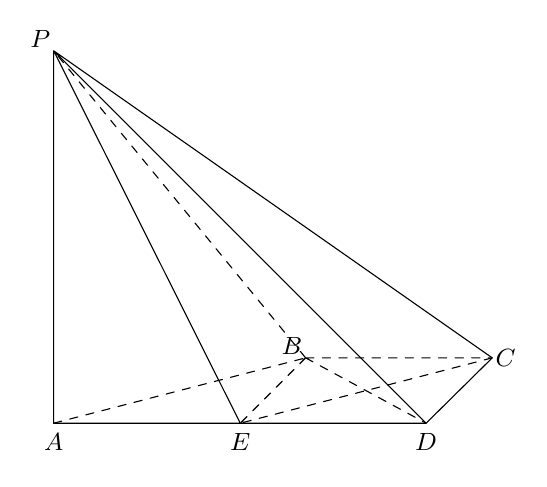
\begin{tikzpicture}[line cap=round,line join=round,font=\small]
\coordinate (P) at (-2.80,4.90);
\coordinate (A) at (-2.80,0.17);
\coordinate (E) at (-0.43,0.17);
\coordinate (D) at (1.93,0.17);
\coordinate (B) at (0.40,1.00);
\coordinate (C) at (2.77,1.00);
% 虚线先画
\draw[dashed] (C)--(E) (A)--(B) (B)--(E) (B)--(C) (B)--(D) (B)--(P);
% 实线后画（压住虚线交叉处，与原图一致）
\draw (A)--(D) (E)--(P) (D)--(P) (C)--(D) (C)--(P) (A)--(P);
\node[above left,inner sep=1pt] at (P) {$P$};
\node[below] at (A) {$A$};
\node[below] at (E) {$E$};
\node[below] at (D) {$D$};
\node[above left,inner sep=1pt] at (B) {$B$};
\node[right,inner sep=1pt] at (C) {$C$};
\end{tikzpicture}
\end{center}
\nopagebreak[4]
（1） 在平面 \(PAB\) 内找一点 \(M\)，使得直线 \(CM\parallel\) 平面 \(PBE\)，并说明理由；

（2） 若二面角 \(P-CD-A\) 的大小为 \(45^{\circ}\)，求直线 \(PA\) 与平面 \(PCE\) 所成角的正弦值。

\end{question}
\begin{question}
\gkti{19}已知数列 \(\{a_{n}\}\) 的首项为 \(1\)，\(S_{n}\) 为数列 \(\{a_{n}\}\) 的前 \(n\) 项和，\(S_{n+1}=qS_{n}+1\)，其中 \(q>0\)，\(n\in\mathbf{N}^{*}\)。

（1） 若 \(2a_{2},a_{3},a_{2}+2\) 成等差数列，求 \(a_{n}\) 的通项公式；

（2） 设双曲线 \(x^{2}-\dfrac{y^{2}}{a_{n}^{2}}=1\) 的离心率为 \(e_{n}\)，且 \(e_{2}=\dfrac{5}{3}\)，证明：\(e_{1}+e_{2}+\cdots+e_{n}>\dfrac{4^{n}-3^{n}}{3^{n-1}}\)。

\end{question}
\begin{question}
\gkti{20}已知椭圆 \(E:\dfrac{x^{2}}{a^{2}}+\dfrac{y^{2}}{b^{2}}=1\)（\(a>b>0\)）的两个焦点与短轴的一个端点是直角三角形的 \(3\) 个顶点，直线 \(l:y=-x+3\) 与椭圆 \(E\) 有且只有一个公共点 \(T\)。

（1） 求椭圆 \(E\) 的方程及点 \(T\) 的坐标；

（2） 设 \(O\) 是坐标原点，直线 \(l'\) 平行于 \(OT\) 与椭圆 \(E\) 交于不同的两点 \(A,B\)，且与直线 \(l\) 交于点 \(P\)，证明：存在常数 \(\lambda\)，使得 \(|PT|^{2}=\lambda|PA|\cdot|PB|\)，并求 \(\lambda\) 的值。

\end{question}
\begin{question}
\gkti{21}设函数 \(f(x)=ax^{2}-a-\ln x\)，其中 \(a\in\mathbf{R}\)。

（1） 讨论 \(f(x)\) 的单调性；

（2） 确定 \(a\) 的所有可能取值，使得 \(f(x)>\dfrac{1}{x}-\mathrm{e}^{1-x}\) 在区间 \((1,+\infty)\) 内恒成立（\(\mathrm{e}=2.718\cdots\) 为自然对数的底数）。

\end{question}